%% Avisa usuario sobre pacotes e versao do LaTeX, nao retire!!!
\typeout{AVISO: ESTE FONTE FOI DESENVOLVIDO UTILIZANDO LaTeX2E!!}
\typeout{PACOTES: SLIDES, BABEL[english,portuguese], INPUTENC(latin1), GRAPHICX}
\typeout{SEM TAIS PACOTES INSTALADOS O FONTE NAO SERA COMPILADO DIREITO!!!}
\typeout{Produzido por Andre Rabello dos Anjos em Setembro de 1997.}
                                                                                                   
\documentclass[a4paper,titlepage]{slides} %% slides class. Also sets for A4 paper type.
                                           
\usepackage[latin1]{inputenc} %% holds ascii as accented chars
\usepackage[french,english,portuguese]{babel} %% sets portuguese as native
\usepackage{graphicx} %% new graphics package
\usepackage{emlines2} %% for pictures
\usepackage{color} %% for colors

%% Include all these
\includeonly{slides/intro, slides/ftmm, slides/project, slides/time, slides/discuss}

%% Title and Authors
\title{Sistema de Classifica��o Baseado em uma M�quina com Processamento Distribu�do}
\author{{\bf \underline{Andr� Rabello dos Anjos}}}

\begin{document}

%% Command definitions
%% Babel stuff
%begin{latexonly}
\newcommand{\eng}[1]{\foreignlanguage{english}{\em{#1\/}}}
\newcommand{\fr}[1]{\foreignlanguage{french}{\em{#1\/}}}
%end{latexonly}

\begin{htmlonly}
\newcommand{\eng}[1]{{\em #1\/}}
\newcommand{\fr}[1]{{\em #1\/}}
\end{htmlonly}

%% shortcuts
\newcommand{\eiro}{$^{\underline{o}}$}
\newcommand{\eira}{$^{\underline{a}}$}
\newcommand{\expo}[2]{$#1^{#2}\/$}
\newcommand{\raw}[1]{{\tt #1}}

%% references
\newcommand{\tabr}[1]{\ref{tab:#1}}
\newcommand{\eqr}[1]{\ref{eq:#1}}
\newcommand{\figr}[1]{\ref{fig:#1}}
\newcommand{\secr}[1]{\ref{sec:#1}}
\newcommand{\tabl}[1]{\label{tab:#1}}
\newcommand{\eql}[1]{\label{eq:#1}}
\newcommand{\figl}[1]{\label{fig:#1}}
\newcommand{\secl}[1]{\label{sec:#1}}

%% characters
%begin{latexonly}
\chardef\bsl=`\\
%end{latexonly}

\begin{htmlonly}
\newcommand{\bsl}{/}
\end{htmlonly}









\maketitle

%% The slides 
%% This file contains 9 slides
\begin{slide}
O mundo sub-at�mico conhecido

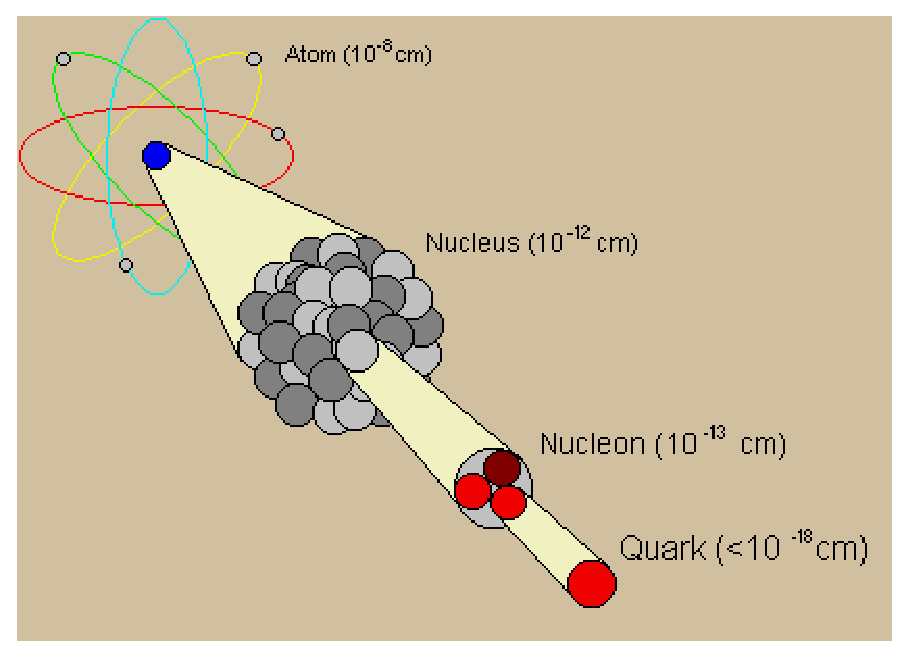
\includegraphics[type = eps, ext = .eps, scale = 1, bb = 0 0 420 300]{figs/atomo}
\end{slide}

\begin{slide}
\begin{center}
O Big-bang

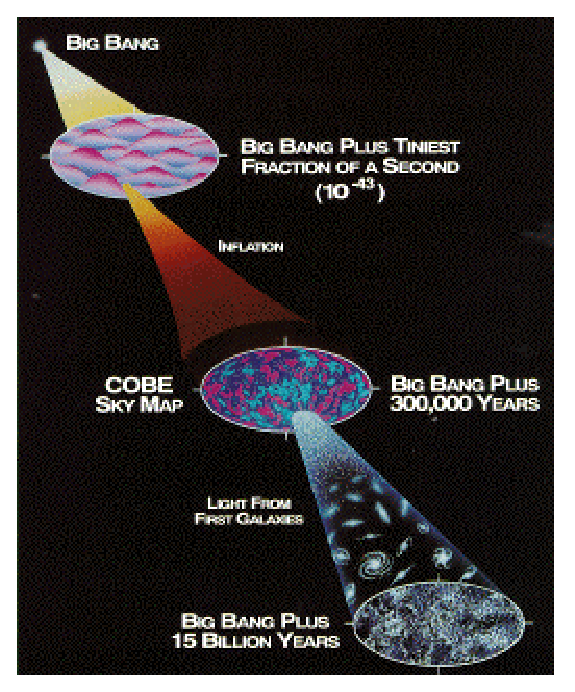
\includegraphics[type = eps, ext = .eps, scale = 1, bb = 0 0 260 316]{figs/bang}                

Os an�is aceleradores do CERN


\includegraphics[type = eps, ext = .eps, scale = 1, bb = 0 0 248 149]{figs/lhcair}
\end{center}
\end{slide}

\begin{slide}
O detetor ATLAS

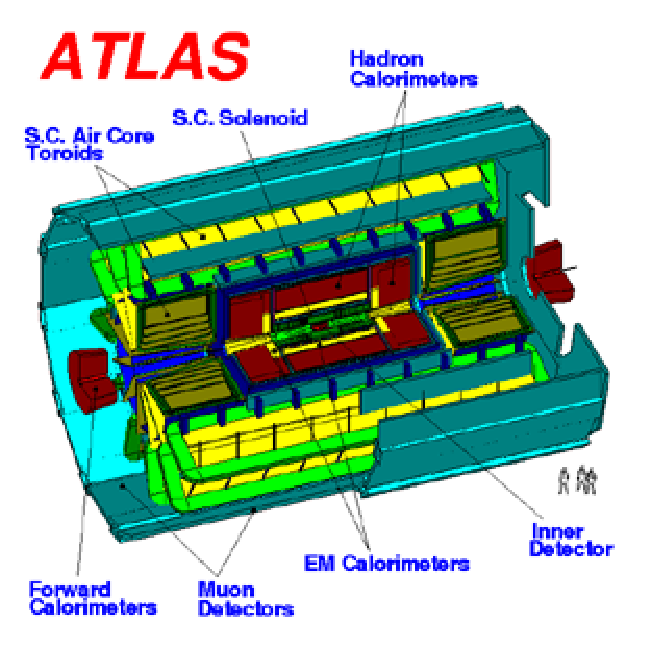
\includegraphics[type = eps, ext = .eps, scale = 1, bb = 0 0 300 295]{figs/atlasair}

Um evento reconstru�do

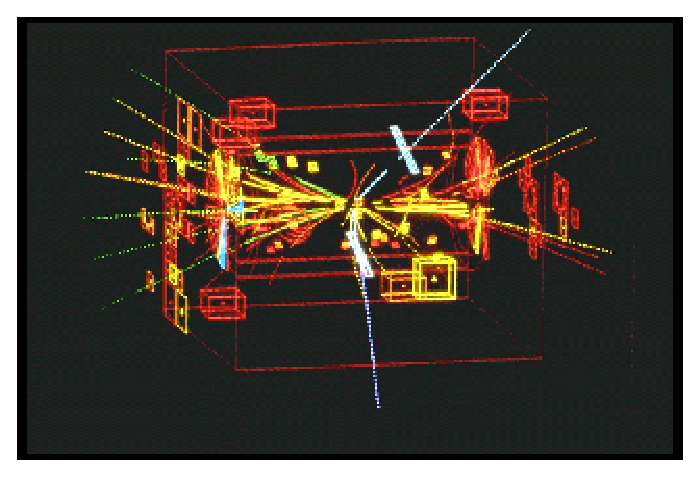
\includegraphics[type = eps, ext = .eps, scale = 1, bb = 0 0 320 213]{figs/colision}
\end{slide}

\begin{slide}
\begin{center}
Porque utilizar sistemas de valida��o ?

$\Downarrow$

Grande volume de dados

$\Downarrow$

\textcolor{blue}{\underline{Inviabilidade}} de armezenar tudo

$\Downarrow$

\textcolor{red}{\underline{Impossibilidade}} de faz�-lo
\end{center}
\end{slide}

\begin{slide}
O Sistema de \eng{Trigger} para o ATLAS

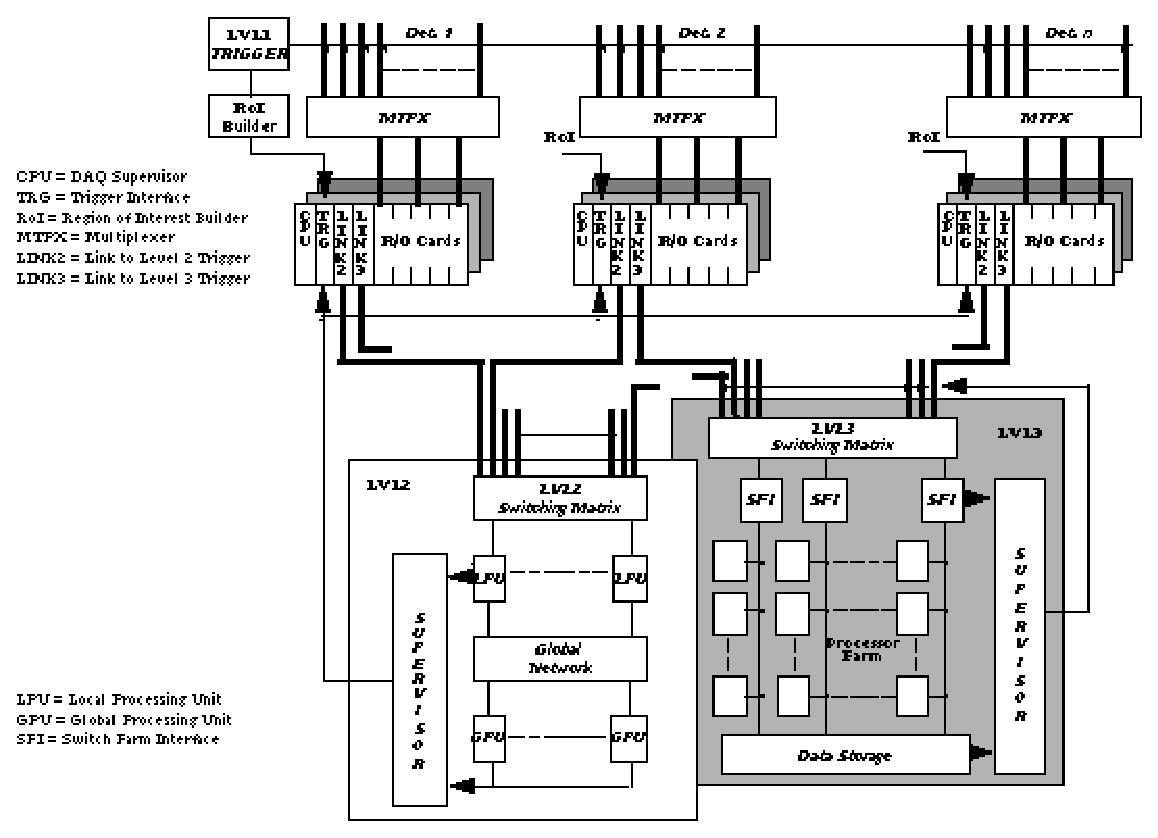
\includegraphics[type = eps, ext = .eps, scale = 0.8, bb = 0 0 540 386]{figs/trigger}
\end{slide}

\begin{slide}
Excitando os detetores

\input{picts/roi2.pic}
\end{slide}

\begin{slide}
A arquitetura A

{\tiny \input{picts/model_a2.pic}}
\end{slide}

\begin{slide}
A arquitetura B

{\tiny \input{picts/model_b2.pic}}
\end{slide}

\begin{slide}
A arquitetura C

{\tiny \input{picts/model_c2.pic}}
\end{slide}


 %% Introduction slides
%% This file contains 6 slides
\begin{slide}
Redes Neurais Artificiais - O neur�nio artificial

\begin{center}
{\tiny \input{picts/neuronc.pic}}
\end{center}
RNA multi-camadas

\begin{center}
{\tiny \input{picts/multi.pic}}
\end{center}
\end{slide}

\begin{slide}
O Sistema TN310

\begin{itemize} 
 \item Processamento Distribu�do
 \item 16 n�s independentes
 \item Mem�ria Local (MIMD)
 \item HTRAM-s tamanho 4
 \begin{enumerate} 
  \item T9000
  \item ADSP 21020 (196Kbytes)
  \item 8Mbytes RAM
  \item 256Kbytes \eng{shared}
 \end{enumerate}
 \item Totalmente conectado atrav�s de chaves STC104
\end{itemize}
\end{slide}

\begin{slide}
O T9000

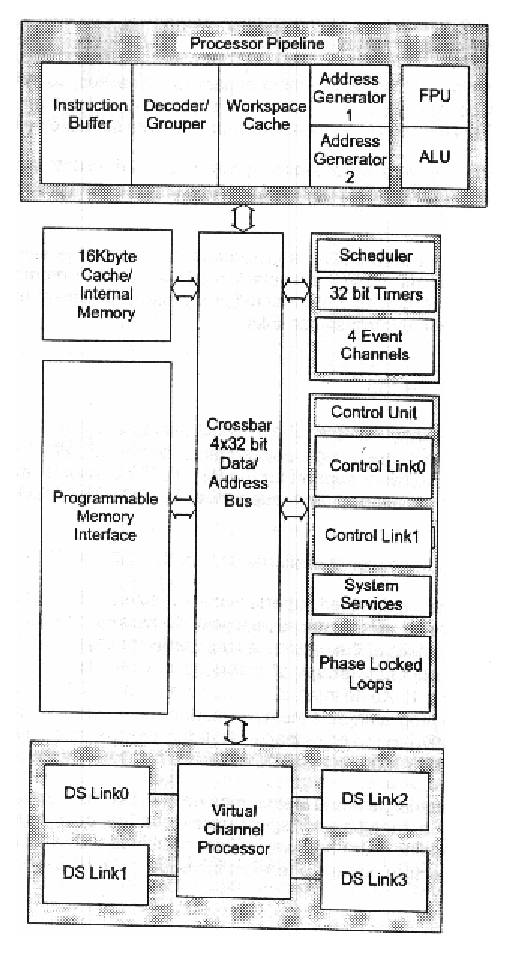
\includegraphics[type=eps, ext=.eps, bb= 0 0 228 441]{figs/T9000}
\end{slide}

\begin{slide}
O ADSP 21020

\end{slide}

\begin{slide}
A conex�o entre os n�s na TN310

{\tiny \input{picts/connect2.pic}}
\end{slide}

\begin{slide}
N�veis de programa��o

\begin{center}
{\tiny \input{picts/layer.pic}}
\end{center}

Comunica��o por canais
\begin{center}
{\tiny \input{picts/chan_op2.pic}}
\end{center}
\end{slide}


 %% Theoretical Fundaments, Methods and Materials slides
%% This file contains 9 slides
\begin{slide}
Modelo de neur�nio utilizado

\begin{center}
{\tiny \input{picts/neuronc.pic}}
\end{center}

A rede para a GDU
\begin{center}
{\tiny \input{picts/gdu_net.pic}}
\end{center}
\end{slide}

\begin{slide}
\begin{center}
Tabela de convers�o

{\tiny \input{picts/lut_ex2.pic}}

GDU em paralelo

{\tiny \input{picts/gdu_full.pic}}
\end{center}
\end{slide}

\begin{slide}
A comunica��o com os escravos

{\tiny \input{picts/shake.pic}}

O supervisor (fluxograma)
z
\begin{center}
{\tiny \input{picts/sup_flow.pic}}
\end{center}
\end{slide}

\begin{slide}
{\small
Resultados para a GDU
\begin{itemize} 
 \item O tempo de processamento para uma RoI da GDU rodando em apenas 1 n� � de 200$\mu$s
 \item Alocando o supervisor no n� zero e 15 escravos o tempo de processamento por 
RoI � de 30,3$\mu$s (\eng{speed-up} = 6.6)
 \item Alocando o supervisor no n� 15 e 15 escravos o tempo de processamento cai 
para 27$\mu$s (\eng{speed-up} = 7.4)
\end{itemize}
Conclus�es
\begin{itemize} 
 \item Tabela de convers�o � eficiente - reduzimos o tempo de processamento sem 
perder efici�ncia
 \item A aloca��o ``inteligente'' de tarefas leva a melhores resultados
 \item \eng{speed-up} - Bom desempenho, mas � o m�ximo ? 
\end{itemize}}
\end{slide}

\begin{slide}
� implementar no 2\eiro n�vel

{\tiny \input{picts/mod_bi2.pic}}
\end{slide}

\begin{slide}
Generaliza��o

\begin{center}
{\tiny \input{picts/top_tn.pic}}
\end{center}
\end{slide}

\begin{slide}
\label{slide:implementa}
Implementa��o usando os 16 n�s

{\tiny \input{picts/sim_v2a2.pic}}
\end{slide}

\begin{slide}
Resultados para a vers�o em apenas 1 n�
\begin{itemize} 
 \item N�o leva em considera��o tempo de distribui��o (necess�rio)
 \item Tempo para uma RoI = 1320$\mu$s
\end{itemize}
Resultado para a vers�o concorrente 1 (aloca��o aleat�ria)

$\Rightarrow$ Tempo para uma RoI = 830$\mu$s (\eng{speed-up} = 1,6)

Resultado para a vers�o concorrente 2 (aloca��o ``inteligente'')

$\Rightarrow$ Tempo para uma RoI = 690$\mu$s (\eng{speed-up} = 1,9)

Resultados para a vers�o concorrente 3 (distribui��o sequencial)

$\Rightarrow$ Tempo para uma RoI = 390$\mu$s (\eng{speed-up} = {\bf 3,4 !})
\end{slide}

\begin{slide}
Conclus�es
\begin{itemize} 
 \item Sabendo que \eng{speed-up} m�ximo � 4 ($//$ dados e fluxo) atingimos 85\% do 
m�ximo
 \item Melhora de 43\% da vers�o 3 para a vers�o 2
 \item Considerando 1 e\-ven\-to $\approx$ 5 RoI-s $\Rightarrow$ 2ms\-/\-e\-ven\-to (500Hz)
 \item Lentid�o $\Rightarrow$ Tempo de distribui��o dos dados para fex-s $\Rightarrow$ 96\% do 
tempo total de aplica��o
 \item Atingimos o m�ximo desta tecnologia ?
\end{itemize}
\end{slide}

 %% Implementation, Results and Conclusion slides
%% This file contains ?? slides
\begin{slide}
Caracterizando a rede de comunica��o
\begin{itemize} 
 \item A comunica��o � feita por pacotes em DS Links (multiplexa��o de canais)
 \item Usa chaves ass�ncronas
\end{itemize}
Tabela de transmiss�o de dados
\begin{center}
\begin{tabular}{|r|c|c|c|c|} \hline
 size & type 1 & type 2 & type 3 & type 4 \\ \hline \hline
 1 & 10,2 & 12,1 & 13,8 & 15,5 \\ \hline
 2 & 16,9 & 20,6 & 24,0 & 27,6\\ \hline
 3 & 23,5 & 28,9 & 34,2 & 39,5\\ \hline
 4 & 30,2 & 37,5 & 44,6 & 51,8 \\ \hline
 5 & 37,2 & 46,0 & 54,7 & 63,6 \\ \hline
 7 & 50,5 & 62,9 & 75,3 & 87,6 \\ \hline
 8 & 57,2 & 71,4 & 85,4 & 99,5 \\ \hline
 10 & 70,8 & 88,2 & 106 & 123 \\ \hline
 11 & 77,3 & 96,7 & 116 & 136 \\ \hline
 13 & 90,6 & 114 & 136 & 159 \\ \hline
 15 & 104 & 130 & 157 & 183 \\ \hline
 16 & 111 & 139 & 167 & 195 \\ \hline
\end{tabular}
\end{center}
\end{slide}

\begin{slide}
{\small
Conclus�es
\begin{itemize} 
 \item � poss�vel prever quando um escravo estar� livre (tempo de processamento). 
Calcular os tempos de transmiss�o para que os escravos sempre estejam livres. 
\begin{displaymath}
n = \frac{tempo\ de\ processamento}{tempo\ de\ trasmiss\tilde{a}o\ para\ outros}
\end{displaymath}
 \item No caso da GDU $n = \frac{200}{27} = 7,41 \Rightarrow$ \eng{speed-up} m�ximo
 \item No caso do 2\eiro n�vel $ n = 2 $ satisfaz taxa m�xima
\end{itemize}}
\end{slide}

\begin{note}
Aqui entra o \eng{slide} da implementa��o, que est� feito em camadas, no 
slide~\pageref{slide:implementa}.
\end{note}

\begin{slide}
Conclus�es finais
\begin{itemize} 
 \item A rede de decis�es globais tem \eng{speed-up} m�ximo de 7,4
 \item � capaz de processar uma RoI em 27$\mu$s = 7,4KHz (evento)
 \item Isto n�o satisfaz o ambiente do segundo n�vel, por�m � o m�ximo a ser 
atingido com esta tecnologia
 \item O \eng{speed-up} m�ximo para o 2\eiro n�vel � 3,4
 \item Isto n�o satisfaz o funcionamento para este tipo de processamento, mas tamb�m
 representa o m�ximo desta tecnologia
\end{itemize}
\end{slide}
 %% Emulation and Time Benchmark results slides
\begin{slide}
Extens�es deste trabalho
\begin{itemize} 
 \item Utiliza��o dos DSP-s \eng{on-board}
 \item Aumentar o n�mero de processos por n� de processamento
 \item Incluir pr�-processamento
 \item Incluir a identifica��o do evento na GDU
\end{itemize}
\end{slide}

 %% Discussion slides

\end{document}

